
\section{Introduction}

\begin{frame}
    \frametitle{Description}
    
    Learned autonomous search for a set of targets in a visual environment with a camera.

    \begin{itemize}
        \item Camera perceives limited region of environment.
        \item Moving camera changes visible region.
        \item Detect when targets are visible.
        \item Locate targets in minimum time.
        \item Learn control from sample scenarios.
        \item Use deep reinforcement learning.
        \item Focus on search behavior, simple detection.
    \end{itemize}
\end{frame}

\begin{frame}
    \frametitle{Problem Statement}

    \begin{columns}
        \begin{column}{0.6\textwidth}
            \begin{itemize}
                \item Searched scene \(S \subset \mathbb{R}^d\).
                \item Perceived view \(V \subset S\) in the form of an image.
                \item View can be transformed to new subspace at a cost.
                \item Targets in scene \(\{t_0, \dots t_n\}\), \(t_i \in S\).
                \item Detect when targets are visible, i.e. \(V \cap T \neq \varnothing\). 
                \item Goal:
                \begin{itemize}
                    \item Maximize probability of finding all targets.
                    \item Minimize cost (time).
                    \item NP-complete~\cite{andreopoulos_theory_2009}. % intractable to solve optimally
                \end{itemize}
            \end{itemize}
        \end{column}
        \begin{column}{0.4\textwidth}
            \begin{figure}
                \centering
                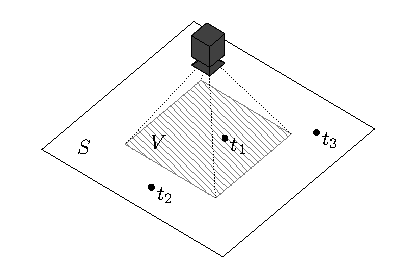
\includegraphics[scale=1.0]{figures/space.pdf}
            \end{figure}
        \end{column}
    \end{columns}   


\end{frame}

\subsection{Motivation}

\begin{frame}
    \frametitle{Motivation}
    
    \begin{itemize}
        \item Applications in search and rescue, surveillance, home assistance, etc.
        \item Autonomous systems may reduce cost and time.
        \item Learning vs. handcrafted systems:
        \begin{itemize}
            \item May find better solutions (deep RL: Atari~\cite{mnih_human-level_2015}, Go~\cite{silver_mastering_2016}, StarCraft II~\cite{vinyals_grandmaster_2019}).
            \item Applicable as long as data is available.
            % Handcrafted systems have to be designed for each specific environment.
            % Learning systems can just be given the problem and some data.
            % Handcrafted systems must be given a solution, which can be difficult to communicate (subtle visual cues).
            % What if we don't know a good solution?
            \item Guarantees and understandability.
        \end{itemize}
    \end{itemize}
\end{frame}

\subsection{Aim}

\begin{frame}
    \frametitle{Aim}
    
    \begin{itemize}
        \item Utilize structure in environments:
        \begin{itemize}
            \item Books are in bookshelves, cars on roads\dots
            \item Targets can be spread out/close together\dots
            % more examples?
        \end{itemize}
        \item Learn distribution of targets from training samples.
        \begin{itemize}
            \item Realistically limited training samples available.
            \item Generalize to similar unseen search scenarios.
        \end{itemize}
        \item Remember features of explored environment to:
        \begin{itemize}
            \item Avoid searching regions twice.
            \item Prioritize promising regions.
        \end{itemize}
    \end{itemize}
\end{frame}

\subsection{Research Questions}

\begin{frame}
    \frametitle{Research Questions}
    \begin{enumerate}
        \item How can an agent that learns to intelligently search for targets be implemented with deep reinforcement learning?
        \item How does the learning agent compare to random, greedy, exhaustive and human searchers?
        \item How well does the learning agent generalize from a limited number of training samples to unseen in-distribution search scenarios?
    \end{enumerate}    
\end{frame}